\documentclass[11pt,a4paper,oneside]{article}
\usepackage[latin1]{inputenc}
\usepackage{amsmath}
\usepackage{amsfonts}
\usepackage{amssymb}
\usepackage{graphicx}
\usepackage{color}
\usepackage {tikz}
\usepackage{fancyvrb}
\usetikzlibrary {er}
\usepackage[left=2.00cm, right=2.00cm, top=1.00cm]{geometry}
\graphicspath{{./}}
\fvset{tabsize=4}

\begin{document}
	\title{DS 255 - System Virtualization \\ Assignment II - Evolution of Virtual Machines}
	\author{Shriram R. \\ M Tech (CDS) \\ 06-02-01-10-51-18-1-15763}
	\maketitle	
	
	\begin{enumerate}
		\item The motivations for using a virtual machine are as follows,
			  \begin{enumerate}
			  	\item To enable server consolidation which leads to reduced hardware and operating costs, improve availability and increase server utilization 
			  	\item To facilitate the execution of multiple versions of privileged software nucleus at the same time in a single bare machine
			  	\item To provide high degree of isolation between machine interfaces to programs. This provides increased system reliability, security and privacy
			  	\item To enable interoperability of software programs that are tied to a specific ISA and OS interface across different systems
			  \end{enumerate}
		      The evolution of Virtual Machine requirements and its impact in system design is detailed below,
		      \begin{enumerate}
		      	\item The requirement of supporting multiple privileged kernels lead to the bare machine to support multiple processor privileged modes natively (more than two) 
		      	\item Virtual machines required to support different ISAs for each application on same OS leading to the creation of ABI virtualization in the form of process VMs. This lead to change in the design of OS to support isolation artefacts such as containers (cgroups) and of compilers to support virtual ISA
		      	\item VMs evolved and needed to support multiple ISAs. This lead to a system design to support emulation of a target ISA in a host ISA with hardware support  
		      	\item The need for hosted VMs (para-virtualization) gave rise to a new design where the host OS provides device drivers and other low level services and the privileged instructions from Guest OS is trapped and handled by the host
		      	\item VMs were required to provide the performance of bare machine along with isolation. This gave rise to the new notion of binding the application code with specific kernel libraries leading to the concept of Unikernels
		      \end{enumerate}	
		      
		\item Basic Machine Interface - It provides access to the execution of both privileged and non-privileged instructions on the bare machine. It is the collection of all software visible objects and instructions that are supported by the hardware and firmware of a system. Note that it can support only one privileged software nucleus directly on top of it.\\
		
		      Extended Machine Interface - The idea behind extended machine interface is to allow for a multiprogrammed environment for user programs with appropriate isolation between them to avoid interference.  The functionalities offered by this interface include the execution of non-privileged hardware instructions and ability to make supervisory (system) calls for privileged functions. \\
		      
		      This extended interface is achieved or realized through the notion of a process. The privileged software nucleus virtualizes the bare machine resources and provides an abstraction of it to each process.
				  
		\item The motivations for server sprawl syndrome are as follows,
		     \begin{enumerate}
		     	\item The need for running each application in isolation by organizations	
		     	\item Unplanned acquisition of large no. of servers to cater to present and future growth
		     	\item Operating System heterogeneity - Example: mail server requiring Windows, database server requiring Linux, network management requiring AIX etc.
		     	\item Relying on coarse grained server driven isolation due to complexity associated with the integration of different applications 
		     	\item Decreasing cost of hardware resources and increasing need for high availability and redundancy accelerated the syndrome  	
		     \end{enumerate}
	          The after effects of this syndrome are as follows,
	          \begin{enumerate}
	          	\item Large number of severely underutilized servers with true utilization in the range of 5-12\% on average in many organizations
	          	\item Increase in Total Cost of Ownership (TCO) (capital + operational expense) due to wastage of resources and large staff required for management
	          	\item Applications were not able to scale effectiviely as per the demand due to 1:1 relationship with the hardware and operating system
	          	\item Increased adoption of server virtualization manifested in data centers to combat this syndrome leading to innovations in virtualization technology   	
	          \end{enumerate}
          
       \item IaaS (Infrastructure as a Service)
             \begin{enumerate}
             	\item The main abstractions/services provided in this layer are the following: Compute, Storage and Networking services. These are available to users as follows,
             	\item The Compute is abstracted as virtual machines for the users generally following different pricing models such as on-demand, prepaid etc.
             	\item The Storage is abstracted as storage pools or buckets which are accessible through APIs, web etc. These are composed of distributed storage systems like SAN in the backend
             	\item The Network is abstracted as virtual network on the cloud. The cloud providers generally offer load balancing, firewall and DNS services as part of Networking infrastructure
                \item IaaS is the delivery of computing infrastructure as a service. It is provisioned and managed over the internet. It provides the highest level of flexibility and management control over the resources. It is the layer above physical hardware
             \end{enumerate}
             PaaS (Platform as a Service)
             \begin{enumerate}
             	\item The main abstractions/services available in this layer are the following: execution runtime, development tools, middleware, database systems etc.
             	\item Note that these services are available in addition to the services from IaaS. Also, some authors/cloud providers consider IaaS and PaaS as a single entity as the accepted defintions for them vary widely
             	\item PaaS abstractions enable efficient application lifecycle management as activities such as capacity planning, patching, software maintenance are taken care by the platform
             	\item Examples of PaaS include Google App Engine, Amazon Beanstalk, Azure SQL etc. 
             \end{enumerate}
             SaaS (Software as a Service)
             \begin{enumerate}
             	\item The main abstractions/services available in this layer are the following: Application software, application data. It is also known as Application service provider (ASP) model
             	\item SaaS offers multi-tenant architecture where the same platform hardware and software is shared among multiple users 
             	\item SaaS enable accessibility to enterprise applications which can scale per demand, automatically perform software updates, etc.
             	\item Examples of SaaS include Salesforce, Microsoft PowerBI, Web mail service etc.
             \end{enumerate} 
         
             The following diagram illustrates the various layers and their abstractions,      
          
	         \begin{center}
	            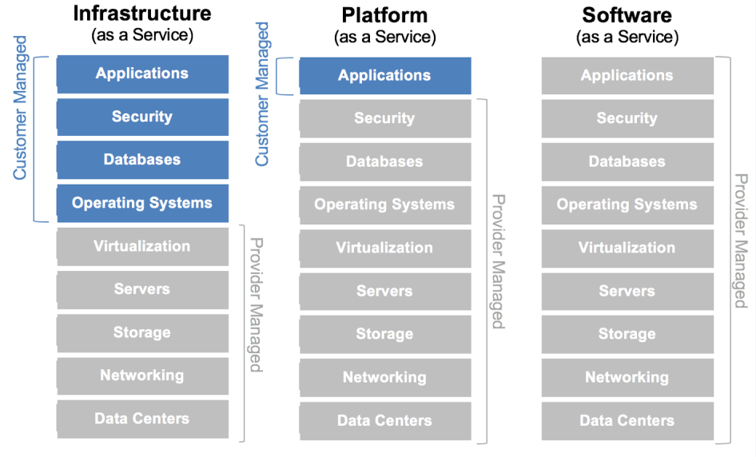
\includegraphics[scale=0.6]{1.png}	[4]
	         \end{center}
         
         
         \item	The cloud differs from normal data centers in the following ways, \\
         
                High Level Differences:
                \begin{enumerate}
                	\item Cloud systems are massively scalable in relative terms. Public clouds are typically distributed globally providing services spanning a large network area
                	\item Cloud systems provide different levels of services to end-users ranging from infrastructure, platform to solutions. The services are designed to be highly dynamic (i.e.) can scale out and scale in based on demand
                	\item It is generally driven by economies of scale and the notion of utility computing provisioning for the end users. Efficient resource utilization is a first class requirement in cloud systems 
                	\item Cloud systems are generally Services oriented as opposed to traditional distributed computing that are Application oriented
                \end{enumerate}
                Resource Management
                \begin{enumerate}
                	\item Resources in cloud are virtually unlimited and typically shared by users at all the time as opposed to dedicated resources governed by queueing system in traditional setup. This allows for running interactive applications on the cloud
                	\item Cloud data storage natively enables data locality for its applications through partitioning, pushing compute to data etc. whereas data centers rely on shared file systems and schedulers to achieve the same goal
                	\item Cloud largely employs virtualization techniques to serve multiple users and applications on demand with efficient resource usage. Traditional data centers generally do not use virtualization mainly for performance reasons
                \end{enumerate}
                Programming and Application Model
                \begin{enumerate}
                	\item Cloud systems have adopted standard web service APISs following HTTP, REST and SOAP protocols and language-agnostic interfaces for coordination and communication while distributed Applications in data centers generally use MPI (Message Passing Interface), RPC (Remote Procedure Call) for coordination between the resources.   
                	\item Applications in data centers are tight-coupled parallel jobs and confined to low latency interconnects. Cloud systems cater to more loosely-coupled and widely distributed applications that are transaction oriented and interactive
                	\item Cloud systems generally use Pay-for-use licenses as opposed to single-purchase licenses generally used in data centers
                \end{enumerate}   	
         
                	
         
         \item	The following points highlight the key rationale behind moving to hyperconverged data centers,
                \begin{enumerate}
                	\item Traditional virtualization methods used in data centers mainly focused on compute therefore leaving storage, networking and data protection outside. This has caused problems for administrators in integrating all the resources efficiently for their applications
                	\item Current data center infrastructure consists of separate, scattered and difficult to scale physical resources like storage, networking etc. which cannot be efficiently pooled and leading to low system utilization. This has lead to inflexibility in provisioning right amount of resources for different applications
                	\item Hyperconverged infrastructure enable agile development environments that can natively support rapid software-release cycles and instantaneous resource provisioning through its unified management layer which was not feasible earlier in the traditional setup
                	\item There is a push towards self-service IT where application developers can provision and manage resources on their own without the need for specialized professional assistance. Software Defined Networking (SDN), Software Defined Data Center (SDDC) etc. can satisfy this requirement
                	\item It enables the paradigm of total virtualization where an entire data center can be treated and priced as an utility. It provides improved control and efficieny. It allows applications to be combined with all its hardware resources to be abstracted as a unified logical application.
                \end{enumerate}
		 			
				
	\end{enumerate}
    
    \textbf{References}
    \begin{enumerate}
    	\item J. P. Buzen and U. O. Gagliardi. 1973. The evolution of virtual machine architecture. In Proceedings of the June 4-8, 1973, national computer conference and exposition (AFIPS '73). ACM, New York, NY, USA, 291-299
    	\item Werner Vogels. 2008. Beyond Server Consolidation. Queue 6, 1 (January 2008), 20-26. 
    	\item G. Khanna, K. Beaty, G. Kar and A. Kochut, "Application Performance Management in Virtualized Server Environments," 2006 IEEE/IFIP Network Operations and Management Symposium NOMS 2006, Vancouver, BC, 2006
    	\item https://www.cs.umb.edu/\textasciitilde marc/cs410/seng10-04.pdf   
    	\item I. Foster, Y. Zhao, I. Raicu and S. Lu, "Cloud Computing and Grid Computing 360-Degree Compared," 2008 Grid Computing Environments Workshop, Austin, TX, 2008
    	\item http://web.mit.edu/smadnick/www/wp/2013-01.pdf	
    	\item http://www.infostor.com/storage-management/hyperconvergence-next-generation-virtualization.html
    	\item https://www.datamation.com/data-center/software-defined-data-centers-could-change-the-it-landscape-1.html
    \end{enumerate}
 

    
\end{document}